\tikzset{every picture/.style={line width=0.75pt}} %set default line width to 0.75pt        

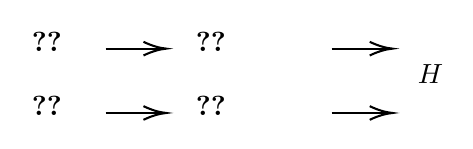
\begin{tikzpicture}[x=0.75pt,y=0.75pt,yscale=-1,xscale=1]
%uncomment if require: \path (0,327); %set diagram left start at 0, and has height of 327

%Straight Lines [id:da29145665996951853] 
\draw [color={rgb, 255:red, 0; green, 0; blue, 0 }  ,draw opacity=1 ]   (53,100) -- (80.23,100) ;
\draw [shift={(82.23,100)}, rotate = 180] [color={rgb, 255:red, 0; green, 0; blue, 0 }  ,draw opacity=1 ][line width=0.75]    (10.93,-3.29) .. controls (6.95,-1.4) and (3.31,-0.3) .. (0,0) .. controls (3.31,0.3) and (6.95,1.4) .. (10.93,3.29)   ;
%Straight Lines [id:da7085137393419103] 
\draw [color={rgb, 255:red, 0; green, 0; blue, 0 }  ,draw opacity=1 ]   (53,131) -- (80.23,131) ;
\draw [shift={(82.23,131)}, rotate = 180] [color={rgb, 255:red, 0; green, 0; blue, 0 }  ,draw opacity=1 ][line width=0.75]    (10.93,-3.29) .. controls (6.95,-1.4) and (3.31,-0.3) .. (0,0) .. controls (3.31,0.3) and (6.95,1.4) .. (10.93,3.29)   ;
%Straight Lines [id:da5772441509961814] 
\draw [color={rgb, 255:red, 0; green, 0; blue, 0 }  ,draw opacity=1 ]   (162,100) -- (189.23,100) ;
\draw [shift={(191.23,100)}, rotate = 180] [color={rgb, 255:red, 0; green, 0; blue, 0 }  ,draw opacity=1 ][line width=0.75]    (10.93,-3.29) .. controls (6.95,-1.4) and (3.31,-0.3) .. (0,0) .. controls (3.31,0.3) and (6.95,1.4) .. (10.93,3.29)   ;
%Straight Lines [id:da8266344132985393] 
\draw [color={rgb, 255:red, 0; green, 0; blue, 0 }  ,draw opacity=1 ]   (162,131) -- (189.23,131) ;
\draw [shift={(191.23,131)}, rotate = 180] [color={rgb, 255:red, 0; green, 0; blue, 0 }  ,draw opacity=1 ][line width=0.75]    (10.93,-3.29) .. controls (6.95,-1.4) and (3.31,-0.3) .. (0,0) .. controls (3.31,0.3) and (6.95,1.4) .. (10.93,3.29)   ;

% Text Node
\draw (95,90.4) node [anchor=north west][inner sep=0.75pt]    {\ref{eq:P3D7_4}};
% Text Node
\draw (16,90.4) node [anchor=north west][inner sep=0.75pt]    {\ref{eq:P3_4}};
% Text Node
\draw (95,121.4) node [anchor=north west][inner sep=0.75pt]    {\ref{eq:P3D7_6}};
% Text Node
\draw (16,121.4) node [anchor=north west][inner sep=0.75pt]    {\ref{eq:P3_6}};
% Text Node
\draw (202,106.4) node [anchor=north west][inner sep=0.75pt]    {$\PIn{H}$};


\end{tikzpicture}
